\documentclass[a4paper,11pt]{article}

\usepackage{amsmath, amssymb, amstext, amsfonts, mathrsfs}


% \sffamily %schrift ohne Serifen

\usepackage[T1]{fontenc} 
% schriftencodierung f�r umlaute, trennung
% f\"ur Uni
\usepackage[latin1]{inputenc}
\usepackage{selinput}
% \usepackage[utf8x]{inputenc} 
\usepackage{bibgerm} 
% german bibliography
\usepackage[german]{babel}
%wichtig f�r deutschen Content
\usepackage{ucs}
%erweiterte UTF-8 Unterst�tzung
\usepackage{wrapfig} 
% Paket zur Positionierung einbinden
\usepackage{multirow}
% zusammenfassen von Tabellenzellen
% \usepackage{subscript}
% zum tiefstellen
\usepackage{lscape}
\usepackage{pdflscape}
% zum drehen der Seite
% \usepackage[super]{natbib}
\usepackage[square,sort,comma,numbers]{natbib}
% Erstellung es Literaturverzeichnisses
\usepackage{url}
% Umbruch f�r URL
\usepackage{pst-3dplot}
% f�r tex Grafiken n�tig
\usepackage{pstricks}
\usepackage{listings}
% f�r das einf�gen von Quelltext
\definecolor{codegray}{rgb}{0.92,0.92,0.92}
\lstset{basicstyle=\fontsize{9}{11}\selectfont\ttfamily, breaklines=true, backgroundcolor=\color{codegray}, numbers=left, numberstyle=\tiny, tabsize=4, language=java}
\definecolor{mymauve}{rgb}{0.58,0,0.82}
\definecolor{mygreen}{rgb}{0,0.6,0}
\lstset{
commentstyle=\color{mygreen},
keywordstyle=\color{mymauve},
language=Java,
stringstyle=\color{blue}
}


%Einstellungen f�r Quellcode
\usepackage[a4paper, left=3cm, right=2cm, top=2cm]{geometry}
% Formatierung R�nder
\usepackage[section]{placeins}
% f�r Floatbarriere
\usepackage{color}
\usepackage{colortbl}
%f�r die Verwendung von Farben

\clubpenalty = 10000 
\widowpenalty = 10000
\displaywidowpenalty = 10000
%Verhinderung von Hurenkindern und Schusterjungen
%10000 bedeutet die sie sollen kommplett vermieden werden

\title{Konzept und prototypische Implementierung eines �bergreifenden Dokumenten- und Medienmanagements als SOA-Anwendung}

\author{Sebastian Rieger}

\pagenumbering{arabic}
%Seitenzahlen(arabische Zahlen)

\setlength{\parindent}{0.25cm} 
%Absatzeinzug �ndern in Zoll
\setlength{\parskip}{0.25cm}
%Absatzabstand
% \linespread {1.1}
%Zeilenabstand

\usepackage{setspace}
\usepackage{hyperref}
%anklickbare Hyperlinks

%funktioniert nicht bei Fu�noten
\usepackage{graphicx}
\usepackage{graphics}
%f�r einbinden von Grafiken

\usepackage{framed}
%f�r Umrandung der Erkl�rung
\usepackage{acronym}
% f�r abk�rzungen
% \usepackage{PSTricks}
\usepackage{epstopdf}
% f�r eps bilder nutze pdflatex --shell-escape this.tex
\usepackage{amssymb}
% f�r mathematische Symbole

\usepackage{hyperref}
% klickbare links

% \usepackage{pdfpages}
\usepackage{rotating}
\usepackage{svg}
%%%%%%%%%%%%%%%%%%%%%%%%%%%%%%%%%%%%%%%%%%%%%%%%%%%%%%%%%%%%%%%%%%%%%%%%%%%%%%%%%%%%%%%%%%%%%%%%%%%%%
%% Angaben zur Arbeit
%%%%%%%%%%%%%%%%%%%%%%%%%%%%%%%%%%%%%%%%%%%%%%%%%%%%%%%%%%%%%%%%%%%%%%%%%%%%%%%

\newcommand{\Autor}{Sebastian Rieger}
\newcommand{\MatrikelNummer}{7406886}
\newcommand{\Kursbezeichnung}{TINF12B1}

\newcommand{\FirmenName}{Karlsruher Institut f�r Technologie (KIT)}
\newcommand{\FirmenStadt}{Karlsruhe}
\newcommand{\FirmenLogoDeckblatt}{{
\includegraphics[width=3cm]{Bilder/kitlogo}}}

% Falls es kein Firmenlogo gibt:
%  \newcommand{\FirmenLogoDeckblatt}{}

\newcommand{\BetreuerFirma}{Dipl. -Inform. Thorsten Schlachter}
\newcommand{\BetreuerDHBW}{Dipl. -Inform., MBA Christian Jordan}
\newcommand{\Titel}{Konzept und prototypische Implementierung eines �bergreifenden Dokumenten- und Medienmanagements}
\newcommand{\AbgabeDatum}{24.08.2015}

\newcommand{\Dauer}{12 Wochen}

% \newcommand{\Abschluss}{Bachelor of Engineering}
\newcommand{\Abschluss}{Bachelor of Science}

\newcommand{\Studiengang}{Angewandte Informatik}
% \newcommand{\Studiengang}{Angewandte Informatik}
\newcommand{\Was}{Bachelorarbeit}

%%%%%%%%%%%%%%%%%%%%%%%%%%%%%%%%%%%%%%%%%%%%%%%%%%%%%%%%%%%%%%%%%%%%%%%%%%%%%%%%%%%%%%%%%%%%%%%%%%%%% 
%steuervariableISO 23081
\usepackage{ifthen} %Package f�r if/else
\newboolean{bilder} %Deklaration
\setboolean{bilder}{true} %Zuweisung
% \setboolean{bilder}{false} %Zuweisung
%%%%%%%%%%%%%%%%%%%%%%%%%%%%%%%%%%%%%%%%%%%%%%%%%%%%%%%%%%%%%%%%%%%%%%%%%%%%%%%%%%%%%%%%%%%%%%%%%%%%%

\begin{document}

\begin{center}
\vspace*{-2cm}
\FirmenLogoDeckblatt\hfill
\includegraphics[width=4cm]{Bilder/dhbw-logo}\\[1cm]
{\Huge \Titel}\\[2cm]
{\Huge\scshape \Was}\\[2cm]
{\large f�r die Pr�fung zum}\\[0.5cm]
{\Large \Abschluss}\\[0.5cm]
{\large des Studienganges \Studiengang}\\[0.5cm]
{\large an der}\\[0.5cm]
{\large Dualen Hochschule Baden-W�rttemberg Karlsruhe}\\[0.5cm]
{\large von}\\[0.5cm]
{\large\bfseries \Autor}\\[1cm]
{\large Abgabedatum \AbgabeDatum}
\vfill
\end{center}
\begin{tabular}{l@{\hspace{1cm}}l}
Bearbeitungszeitraum             & \Dauer                       \\
Matrikelnummer                   & \MatrikelNummer              \\
Kurs                             & \Kursbezeichnung             \\
Ausbildungsfirma                 & \FirmenName                  \\
                                 & \FirmenStadt                 \\
Betreuer der Ausbildungsfirma    & \BetreuerFirma               \\
Gutachter der Studienakademie    & \BetreuerDHBW                \\
\end{tabular}

\newpage
%Seitenumbruch
%%%%%%%%%%%%%%%%%%%%%%%%%%%%%%%%%%%%%%%%%%%%%%%%%%%%%%%%%%%%%%%%%%%%%%%%%%%%%%
%% Descr:       Vorlage für Berichte der DHBW-Karlsruhe, Erklärung
%% Author:      Prof. Dr. Jürgen Vollmer, vollmer@dhbw-karlsruhe.de
%% $Id: erklaerung.tex,v 1.2 2010/07/22 13:30:27 vollmer Exp $
%%%%%%%%%%%%%%%%%%%%%%%%%%%%%%%%%%%%%%%%%%%%%%%%%%%%%%%%%%%%%%%%%%%%%%%%%%%%%%%

% In Bachelorarbeiten muss eine schriftliche Erklärung abgegeben werden. In allen anderen
% Arbeiten entf�llt diese. Hierin best�tigen die Studierenden, dass die Bachelorarbeit
% selbst�ndig verfasst und s�mtliche Quellen und Hilfsmittel angegeben sind. Diese Erkl�rung
% bildet das zweite Blatt der Arbeit. Der Text dieser Erkl�rung muss auf einer separaten Seite
% wie unten angegeben lauten.

\newpage
\thispagestyle{empty}
\begin{framed}
\begin{center}
\Large\bfseries Erkl\"arung
\end{center}

\noindent
Gem\"a\ss{}�16 (3) der "`Studien- und Pr\"ufungsordnung f\"ur den Studienbereich
Technik"' vom 1.11.2007.

\medskip
\noindent
Ich habe die vorliegende Arbeit selbstst\"andig verfasst und
keine anderen als die angegebenen Quellen und Hilfsmittel verwendet.

\vspace{3cm}
\noindent
\underline{\hspace{4cm}}\hfill\underline{\hspace{6cm}}\\
Ort~~~~~Datum\hfill Unterschrift\hspace{4cm}
\end{framed}

%%%%%%%%%%%%%%%%%%%%%%%%%%%%%%%%%%%%%%%%%%%%%%%%%%%%%%%%%%%%%%%%%%%%%%%%%%%%%%%
\endinput
%%%%%%%%%%%%%%%%%%%%%%%%%%%%%%%%%%%%%%%%%%%%%%%%%%%%%%%%%%%%%%%%%%%%%%%%%%%%%%%

\newpage
\begin{spacing}{0.9}

%Einf�gen Inhaltsverzeichnis
\tableofcontents



\end{spacing}

\newpage
\section{Abstract}
\newpage
\section{Einleitung} \label{Einfuehrung}
Beh\"orden und Firmen haben heute immer gr\"o\ss{}ere Datenbest\"ande zu verwalten, welche schon in elektronischen Systemen vorzufinden sind. Da diese Systeme historisch bedingt gewachsen sind, entstanden im laufe der Zeit immer mehr kleinere Insell\"osungen, welche ein \"ubergreifendes Verwalten und Nutzen von Daten erschwert oder gar ganz verhindert.

Das Ziel dieser Arbeit soll es daher sein, ein Konzept sowie eine prototypische Implementierung zu ertsellen, welche ein \"ubergreifendes und vereinheitlichtes arbeiten mit den Datenbest\"anden erm\"oglicht. Heutige \ac{DMS} Systeme decken eine vielzahl von Anwendungsgebieten ab, welche an die jeweiligen Problemstellungen wie Rechtsfragen oder fachliche Anforderungen angepasst sind oder angepasst werden k\"onnen.
Ein genaues Konzept mit Anforderungen, soll am Beispiel der \ac{LUBW} sowie der \ac{GAA} entstehen.
\cite{Dokumenten-Management}

Es sollen durch das Konzept auch bestehende Systeme weiter unterst\"utzt werden, wof\"ur hier eine Anbindungsm\"oglichkeit geschaffen werden soll. \"Uber eine serviceorientierte Anbinung sollen somit die verschiedensten Frontends wie Desktopanwendung, Web, Mobil usw. das neue Konzept nutzen k\"onnen. Welches \ac{ECM}-Tool f\"ur die Erstellung des Projekts am besten geeignet ist, muss analysiert werden, ergibt sich jedoch aus den zu verwaltenden Dokumenten.

F\"ur die Arbeit soll hierbei kein komplett neues \ac{DMS} mit Nutzer und Dokumentverwaltung entwickelt werden. Vielmehr soll evaluiert werden, welche Systeme es bereits auf dem Markt gibt, und wie sich diese f\"ur die anstehnde Aufgabe eignen, vor allem im Bezug auf die hierachische Gliederung der Metadaten, wie im Projekt vorgesehen ist. 

Als sogenannter \ac{PoC} soll im Verlauf dieser Arbeit ein bestehendes Fachsystem auf der Basis einer erarbeiteten Schnittstelle nachgebaut werden. Diese Frontend soll das derzeitige \ac{FADO}-System der \ac{LUBW} nachbilden.
\newpage
\section{Lastenheft} \label{Lastenheft}
An das Projekt, welches im Rahmen dieser Arbeit bearbeitet werden soll, gibt es viele Anforderungen. Um alle Anforderungen m\"oglichst strukturiert und \"Ubersichtlich darzustellen, wurde die Form eines Lastenhefts gew\"ahlt.

\subsection{Zielsetzung} \label{Zielsetzung}
Ziel ist es ein einheitliches \ac{ECM} System zu entwerfen, welches m\"oglichst alle Fachdokumente der \ac{LUBW} und der \ac{GAA} beinhaltet.
Hierbei sollen alle bestehenden und zuk\"unfitgen Systeme \"uber eine Schnittstelle mit dem \ac{DMS} kommunizieren.

\subsection{Produkteinsatz} \label{Produkteinsatz}
Bei dem zu entwickelnden System, handelt es sich um einen Prototyp f\"ur ein \ac{DMS}, welches gegebenenfalls von der \ac{LUBW} und der \ac{GAA} eingesetzt werden kann. Das zu entwickelnde Backend, soll alle Dokumente, welche schon heute auf den Websiten zu finden sind zusammenf\"uhren und diese in einer geeigneten Form ablegen.

\subsubsection{Zusammenspiel mit anderen Systemen} \label{Zusammenspiel mit anderen Systemen}
Das Backend soll nicht die heutigen Insell\"osungen f\"ur Dokumentverwaltung der \ac{LUBW} und der \ac{GAA} vereinen. Es sollen sowohl die bestehenden als auch zuk\"unfitge Systeme unterst\"utzt werden. Die jeweils ben\"otigten Daten, sollen hierf\"ur \"uber eine oder gegebenenfalls mehrere Schnittstellen erreichbar sein.

\subsection{Produktfunktionen} \label{Produktfunktionen}
\begin{minipage}{3cm}
/LF10/
\end{minipage}
\begin{minipage}{13cm}
Schon bestehende Dokumente sollen aus den alten Systemen \"ubernommen werden k\"onnen, ohne das ihre Metadaten verloren gehen oder ge\"andert werden. Dies bedeutet, dass das neue System den schon vorhandenen Datenbestand abbilden muss.\\
\end{minipage}
\begin{minipage}{3cm}
/LF20/
\end{minipage}
\begin{minipage}{13cm}
Die Metadaten der einzelnen Dokumente sollen fachlich und technisch gegliedert werden. Hierbei sollen gegebenenfalls Gruppierungen erstellt werden. Zum Beispiel sollen Longitude und Latitude zur Metadaten-Gruppe "`Geodata"' zusammengefasst werden.\\
\end{minipage}
\begin{minipage}{3cm}
/LF30/
\end{minipage}
\begin{minipage}{13cm}
Die Dokumente sollen ebenfalls nach den einzelnen Anwendungen und Fachbereichen gruppiert werden. Hier sollen die Anwendungen auch speziell ihre Dokumente nach Gruppenzugeh\"origkeit abfragen k\"onnen. Dies ist wichtig, da im \ac{FADO} nur die entsprechenden \ac{FADO}-Dokumente angezeigt werden sollen.\\
\end{minipage}
\begin{minipage}{3cm}
/LF40/
\end{minipage}
\begin{minipage}{13cm}
Eine Suche \"uber die Dokumente und ihre Metadaten soll grunds\"atzlich m\"oglich sein. Hier muss der Nutzer aber auch in der Lage sein die Suche weiter einzuschr\"anken oder nur nach bestimmten Metadaten suchen zu k\"onnen.\\
\end{minipage}
\begin{minipage}{3cm}
/LF50/
\end{minipage}
\begin{minipage}{13cm}
Die alten Systeme sollen durch das neue Backend keinerlei Einschr\"ankungen im Funktionsumfang unterworfen sein. Dies muss gegebenenfalls durch verschiedene Arten von Schnittstellen realisert werden.\\
\end{minipage}
\begin{minipage}{3cm}
/LF60/
\end{minipage}
\begin{minipage}{13cm}
F\"ur den Frontend-Prototyp, soll die Kernfunktionalit\"at einer Schnittstelle funktionsf\"ahig sein, anhand dessen der Prototyp evaluiert werden kann.\\
\end{minipage}

\subsection{Produktdaten} \label{Produktdaten}
\begin{minipage}{3cm}
/LD10/
\end{minipage}
\begin{minipage}{13cm}
Die entsprechenden Metadaten zu Dokumenten sollen durch das Backend verwaltet werden. Hierbei sollen nicht nur die manuell hinzugef\"ugten Metadaten beachtet werden, sondern auch die Metadaten, welche das Dateiformat liefert und solche die das Dokument enth\"alt.\\
\end{minipage}
\begin{minipage}{3cm}
/LD20/
\end{minipage}
\begin{minipage}{13cm}
Metadaten sollen nach M\"oglichkeit so zusammengefasst werden, das eine Oberklassenbildung und Vererbung von Metadaten m\"oglich ist. So soll zum Beispiel ein Standort alle Adressdaten zusammenfassen. Ein Standort wiederum kann in mehreren Dokumenten verwendet werden, wie zum Beispiel in Bildern oder in einem Forschungsbericht. Wiederum k\"onnte der Standort aber auch Betandteil der Unterklasse Gericht sein und somit den Standort des Gerichts abbilden.\\
\end{minipage}
\begin{minipage}{3cm}
/LD30/
\end{minipage}
\begin{minipage}{13cm}
Metadaten sollen \"ahnlich wie objektorientierte Klassen in Programmiersprachen agieren. So wird ein Autor "`Max Mustermann"' nur einmal angelegt. Er kann jedoch in mehreren Dokumenten auftauchen. Sucht ein Nutzer nach "`Max Mustermann"', so werden ihm alle Eintr\"age zu diesem angezeigt. Vergleichen kann mal diese Art von Abbildung auch mit einer relationalen Abbildung wie sie in Datenbanken zu finden ist.\\
\end{minipage}
\begin{minipage}{3cm}
/LD40/
\end{minipage}
\begin{minipage}{13cm}
F\"ur die Gliederung der Metdaten sollen auch schon bestehende Standards betrachtet und gegebenenfalls umgesetzt werden.
Im Verlauf der Arbeit muss evaluiert werden, welche Standards es f\"ur Metadaten gibt und wie sie im Projekt umgesetzt werden m\"ussen und k\"onnen.
\cite{Wiki_Dublin_Core} \cite{Wiki_ISO_19115} \cite{Wiki_Exif} \cite{Wiki_Inspire}\\
\end{minipage}


\subsection{Produktleistungen} \label{Produktleistungen}
\begin{minipage}{3cm}
/LL10/
\end{minipage}
\begin{minipage}{13cm}
Das Backend soll f\"ur Dokumente, welche in verschiedenen Versionen vorliegen eine Art Versionsverwaltung bieten, so das auch \"altere Versionen zug\"anglich sind. Dies zum Beispiel bei Gesetzestexten wichtig, da hier immer die zum Vorfall aktuelle Version betrachtet werden muss.\\
\end{minipage}
\begin{minipage}{3cm}
/LL20/
\end{minipage}
\begin{minipage}{13cm}
Die Dokumente sollen \"uber verschiedene Schnittstellen wie zum Beispiel eine \ac{REST}-Schnittstelle abgerufen werden k\"onnen. Der Einsatz von \ac{API}s ist je nach \ac{ECM}-Tool gegebenenfalls auch m\"oglich, jedoch ist eine solche Ums\"atzung nicht Teil der Arbeit. \cite{Wiki_REST}\\
\end{minipage}
\begin{minipage}{3cm}
/LL30/
\end{minipage}
\begin{minipage}{13cm}
Eine Suche \"uber Metadaten muss realisert werden. Hierbei soll dem Nutzer zum einen eine grobe aber auch zum anderen eine verfeinerte eingeschr\"ankte Suche nach bestimmten Metadaten geboten werden.\\
\end{minipage}
\newpage
\section{Stand der Technik / existierende Konzepte} \label{Stand der Technik}
Im folgenden Kapiel werden die einzelnen Fachsysteme, der \ac{LUBW} und deren Datenbest\"ande genauer analysiert. Zus\"atzlich wird ein Blick auf das Literaturarchiv der \ac{ICT-ENSURE} gerichtet, um ein m\"oglichst \"ubergreifendes Metadatenmodell erstellen zu k\"onnen. 

Welche Metdaten die einzelnen Dokumentenbest\"ande der Fachsysteme genau enthalten ist im Anhang \ref{Metadaten der LUBW Fachsysteme} genau aufgelistet. Hierbei wird unterschieden, ob es sich um Metadaten oder relationen handelt. Daf\"ur wurden alle Metadaten aus den Systemen extrahiert.


Die Metadaten der in diesem Kapitel untersuchten Systeme werden anschlie\ss{}end im Kapitel \ref{Erstellung eines Datenkonzepts} zu einem \"ubergreifenden Metadatenmodell vereint, welches die sp\"atere Grundlage f\"ur ein \ac{ECM}-Tool sein soll.

% Die einzelnen Fachsysteme der \ac{LUBW} sind f\"ur unterschieliche Einsatzzwecke entwickelt wurden, welche nun genauer anlaysiert werden.
% Ebenso wird das Literaturarchiv der \ac{ICT-ENSURE} untersucht, um ein \"ubergreifendes Datenmodell zu erstellen.

\subsection{FADO und Untergruppen} \label{FADO}
Das \ac{FADO}-System der \ac{LUBW} erlaubt es den Nutzern nach verschiedenen Texten aus unterschielichen Themenrichtungen zu suchen und diese herunterzuladen. Hierbei stehen die Dokumente, zum Teil wahlweise, im PDF- oder HTML-Format bereit.

Die einzelnen Ver\"offentlichungen k\"onnen nach verschiedenen Kriterien durchsucht werden, wobei der Bestand an Dokumenten, von der \ac{LUBW} fortlaufend erweitert wird.
\cite{LUBW_FADO}

Im \ac{FADO}-System sind die Dokumente in die sechs Kategorien Altlasten, Boden, Natur und Landschaft, Umweltbeobachtung, Umweltforschung und Umweltinformationssysteme gegliedert. Hierbei ist zu beachten, dass ein Dokument nicht nur einem Themengebiet zugeordent werden kann, sondern durchaus unter mehreren Gebieten zu finden ist. Solche Dokumente sind im \ac{FADO} jedoch nur einmal abgespeichert und werden \"uber Relationen den verschiedenen Kategorien zugeordent.

Die einzelnen Kategorien sind wiederum mit Untergruppen versehen, welche die Zugeh\"origkeit der Dokumente konkretisieren.

Da im Verlauf der Arbeit nicht alle Gruppen in ein neues System \"uberf\"uhrt werden k\"onnen, wird sich auf die Dokumentklassen Berichte, Urteile und Forschungsvorhaben beschr\"ankt, welche in der Kategorie Natur und Landschaft, in der Kategorie Boden beziehungsweise in der Kategorie Umweltforschung zu finden sind.

Forschungsvorhaben wiederum sind Berichte, welche sich in eine Skizze, einen Zwischen- und einen Abschlussbericht aufteilen. Hierbei geh\"oren die drei Teile zu jeweils einem Forschungsvorhaben. \cite{LUBW_FADO}

\subsection{Das Document Retrieval System} \label{DRS}
Das \ac{DRS} der \ac{LUBW} ist eine Art Suchmaschine, die es erm\"oglicht verschiedene Rechtsvorschriften, Regelungen, Fachberichte und Erl\"asse zu suchen. Abfragen im \ac{DRS} k\"onnen auf drei Arten erfolgen. Es gibt die "`Standardsuche"', welche es erlaubt nach Inhalt oder Metadaten der Dokumente zu suchen. Die "`Titelsuche"' erlaubt es, wie der Name schon sagt nach Titeln oder gegebenenfalls nach Normtiteln der Dokumente zu schauen. Als dritte M\"oglichkeit bietet das \ac{DRS} eine "`Geziehlte Suche"' an, die es erm\"oglicht Suchkriterien genau anzugeben und diese auch einzuschr\"anken.
\cite{DRS}

Zu beachten ist, dass das \ac{DRS} eine eigenst\"andiges Plattform ist, welche einen eigenen Dokumentenbestand vorh\"alt.

In Abbildung \ref{Suchmaske DRS} ist die Suchmaske der "`Geziehlten Suche"' vom \ac{DRS} zu sehen. Es werden in der Maske alle M\"oglichkeiten aufgef\"uhrt, nach denen gesucht werden kann, was alle vorhandenen Metadaten mit einschlie\ss{}t. Die meisten Metadaten, sind durch Auswahllisten beschr\"ankt und andere k\"onnen vom Nutzer frei mit Begrifflichkeiten gef\"ullt werden.

Zu sehen ist in den Feldern Fassung und \"Anderung, dass eine Art Verwaltung von \"alteren Versionen vorgenommen wird. Diese Versionierung ist notwendig, da alte Gesetzestexte f\"ur in der Vergangenheit liegende F\"alle aufbewahrt werden m\"ussen.

\begin{figure}[!ht]
\centering
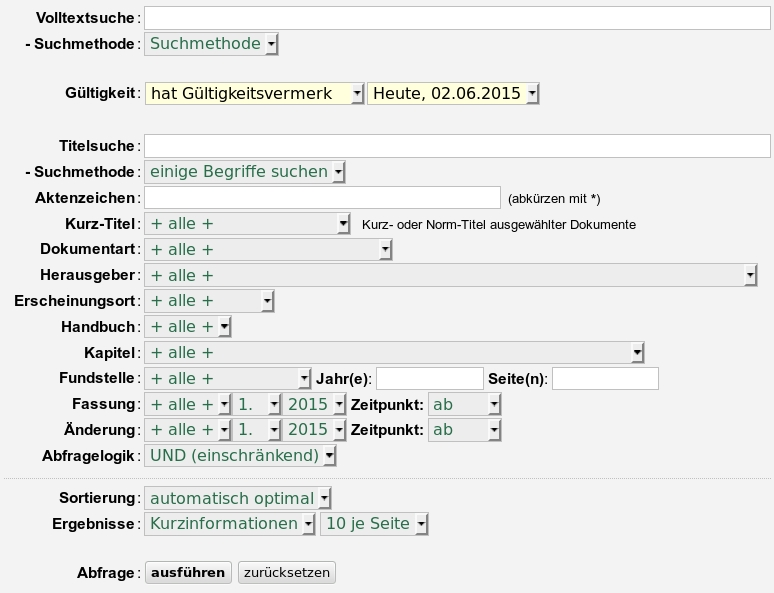
\includegraphics[width=15cm]{Bilder/Suchmaske_DRS.jpg}
\caption{Suchmaske des \ac{DRS}}
\label{Suchmaske DRS}
\centering
\end{figure}

\subsection{Naturschutz-Bildarchiv} \label{Bilddatenbank}
Im Naturschutz-Bildarchiv der \ac{LUBW} finden sich viele Bilder zu verschiedenen Themengebieten, so zum Beispiel auch zu den Gebieten Biotoptyp, Lebensraumtyp, Naturschutzgebiet und einige mehr.
\cite{Naturschutz-Bildarchiv}

Diese Themenkomplexe k\"onnen wiederum nach Stichworten durchsucht werden, wie zum Beispiel "`Aurorafalter"', was im Themengebiet "`Pflanzen- und Tierart"' Bilder von entsprechenden "`Faltern"' liefert. Auch das Bildarchiv ist ein eigenst\"andiges System, welches seinen eigenen Dokumentenbestand besitzt.

\subsection{Literaturarchiv der ICT-ENSURE}
Im Literaturarchiv der \ac{ICT-ENSURE} sind verschiedene Dokumente zu verschiedenen Themengebieten zu finden. Die \ac{ICT-ENSURE} ist ein EU-Projekt, welches es sich zur Aufgabe gemacht hat die Zusammenarbeit von Forschung und Wissenschaft in Europa zu st\"arken.

\ac{ICT-ENSURE} enth\"alt wie schon erw\"ahnt viele verschiedene Dokumente aus dem Breich Forschung und erlaubt eine Volltextsuche innerhalb dieser Dokumente. Zus\"atzlich sind die einzelnen Dokumente nach verschiedenen Fachrichtungen beziehungsweise Konferenzen gegliedert.
\cite{ICT-ENSURE_Bericht}

Alle Dokumente der \ac{ICT-ENSURE} sind B\"ucher, und so erfolgt auch ihre Speicherung.
Zu jeder Konferenz gibt es ein Buch, welches in Kapitel unterteilt ist. Diese Kapitel wiederum sind in Unterkapitel geteilt, welche den einzelnen Vortr\"agen entsprechen.

Eine genaue Auflistrung der Metadaten ist im Anhang \ref{Metadaten der ICT-ENSURE} zu finden.

\newpage
\section{Analyse von Metadatenstandards} \label{Analyse Datenbestaende}
Nach dem nun die Portale \ac{DRS}, Naturschutz-Bildarchiv und \ac{FADO}, der \ac{LUBW} und das Literaturarchiv der \ac{ICT-ENSURE} im Kapitel \ref{Stand der Technik} genauer betrachtet und die Verwaltungsstrukturen aufgezeigt wurden, betrachtet dieses Kapitel nun Standards f\"ur Metadaten. Hierbei wird unterschieden, ob es sich um fachliche oder technische Metadaten handelt.

\subsection{Fachlich}
Fachliche Metadaten sind Daten, welche den Inhalt einer Datei oder eines Dokuments genauer beschreiben und dem Anwender dabei helfen f\"ur ihn relevante Dateien zu identifizieren. Solche Metadaten sind immer fachspezifisch und unabh\"angig von den technischen Eigenschaften einer Datei.
\cite{Fachliche_Metadaten_Wissensportal_BI} \cite{Fachliche_Metadaten_msg} \cite{DHW_Wiki_Metadaten} \cite{Multimedia_retrieval}

Die Dokumente der Fachsysteme der \ac{LUBW}, sowie der \ac{ICT-ENSURE} enthalten alle fachliche Metadaten. Eine genaue Aufstellung aller fachlichen Metadaten der in dieser Arbeit untersuchten Dokumente ist im Anhang \ref{Metadaten der LUBW Fachsysteme} zu finden.

\subsection{Fachliche Metadaten-Standards} \label{Fachliche Metadaten-Standards}
F\"ur die Erstellung eines Datenkonzepts wie es im Kapitel \ref{Erstellung eines Datenkonzepts} geschieht, ist es aber nicht nur notwendig die vorhandenen Metadaten zu betrachten. Auch Standards f\"ur fachliche Metadaten sollen in diesem Umfeld untersucht werden.

Da fachliche Metadaten meist anwendungs- beziehungsweise dokumentbezogen sind, gibt es nicht sehr viele Standards, welche sich im Umfeld der \ac{LUBW} beziehungsweise der \ac{ICT-ENSURE} einsetzen lassen.

\subsubsection{Darwin Core}\label{Darwin Core}
Darwin Core beschreibt eine Zusammenfassung von Metadaten, welche f\"ur biologische Zwecke eingesetzt werden k\"onnen. So ist es zum Beispiel m\"oglich, Angaben zum Organismus oder zum Lebensraum zu machen. 

Hierf\"ur verwendet Darwin Core bis zu 172 Tags, welche jedoch nicht zwingend verwendet werden m\"ussen. Zus\"atzlich enth\"alt der Standard auch die Tags von Dublin Core (siehe Abschnitt \ref{Dublin Core}) um das Dokument grundlegend zu beschreiben.
\cite{Darwin_Core} \cite{Wiki_Darwin_Core}

Ii Listing \ref{Darwin Core Beispiel in XML}\footnote{\url{http://rs.tdwg.org/dwc/terms/guides/xml/index.htm}} ist einmal ein Beispiel f\"ur den Darwin Core-Standard  mit XML dargestellt. Es ist zu sehen, das ein "`SimpleDarwinRecord"' verwendet wird, welcher nicht alle 172 Tags beinhaltet. 

Es ist auch zu erkennen, dass die Dublin Core-Tags inbegriffen sind (beginnend mit "`dcterms"'). Die eigentliche Tags des Darwin-Standards beginnen mit "`dwc"'.
\lstinputlisting[caption=Darwin Core-Beispiel in XML, label=Darwin Core Beispiel in XML]{Code/Darwin_Core.xml}

\subsubsection{INSPIRE} \label{INSPIRE}
\ac{INSPIRE} ist ein Standard f\"ur Metadaten, welcher von der \ac{EU} nach der Richtlinie "`2007/2/EG"' vom 14. M�rz 2007 erlassen wurde. \ac{INSPIRE} enth\"alt Metadaten, welche f\"ur Geo-Referenzen benutzt werden m\"ussen, denn nach der eben genannten \ac{EU}-Richtlinie m\"ussen alle vom Land ver\"offentlichten digitalen Dateien mit Geo-Referenzen versehen werden.

\ac{INSPIRE} stellt 25 Meta-Tags zur Verf\"ugung, mit dessen Hilfe die \ac{EU}-Richtlinie zur Bekanntmachung von Geo-Referenzen eingehalten wird.
Au\ss{}erdem enth\"alt der \ac{INSPIRE}-Standard die notwendigen Tags der DIN EN ISO 19115 (siehe Abschnitt \ref{ISO 19115}), wodurch dieser gleichzeitig nach dieser Norm ISO-konform wird. 
\cite{INSPIRE_Richtlinie}

Von den 25 Meta-Tags m\"ussen 12 Tags zwingend angegeben werden, um die Richtlinie zu erf\"ullen. Die Meta-Tags von \ac{INSPIRE} sind zum Teil untergliedert, was bedeutet, dass eine Vielzahl mehr an Information in diesen Standard enthalten sein k\"onnen.

Aus \"Ubersichlichkeitsgr\"unden wird an dieser Stelle kein Beispiel Listing erfolgen, da das XML-Format von \ac{INSPIRE} sehr ausf\"uhrlich und gro\ss{} ist. Es wird jedoch an dieser Stelle auf den Editor f\"ur \ac{INSPIRE}-Metadaten der Europ\"aischen Kommission verwiesen, mit dessen Hilfe schnell und einfach XML-Dokumente mit \ac{INSPIRE}-Metadaten erzeugt werden k\"onnen\footnote{\url{http://inspire-geoportal.ec.europa.eu/editor/}}.
\cite{INSPIRE_Geoportal} \cite{Wiki_Inspire} 

\subsubsection{DIN EN ISO 19115} \label{ISO 19115}
Die DIN EN ISO 19115 ist eine Norm, welche 2005 spezifiziert wurde. Sie enth\"alt Metadaten f\"ur die Bescheibung von Geo-Information. Mit \"uber 400 m\"oglichen Tags ist sie eine der detailliertesten Beschreibungsstandards f\"ur Geo-Daten. 

Von den \"uber 400 Tags sind f\"ur eine Verwendung der Norm nur ca. 22 Tags erforderlich. Alle anderen Tags sind optional.
\cite{ISO_19115_Doku} \cite{Wiki_ISO_19115}

Wird der \ac{INSPIRE}-Standard verwendet (siehe Abschnitt \ref{INSPIRE}), so ist automatisch auch die ISO 19115 erf\"ullt, da diese Bestandteil  von \ac{INSPIRE} ist.
\cite{INSPIRE_Richtlinie}

\subsubsection{ONIX}
Der \ac{ONIX}-Standard ist international bekannt und f\"ur den elektronischen Austausch von Buchinformationen geschaffen worden.

\ac{ONIX} kann gem\"a\ss{} der Lizenz frei verwendet werden und ist zur Beschreibung von traditionellen B\"uchern und E-Books vorgesehen.
Der Standard enth\"alt sehr viele Tags, mit dessen Hilfe ein Buch beschrieben werden kann. So k\"onnen zum Beispiel Angaben zum Verleger und zur ISBN gemacht werden. \cite{ONIX} \cite{Wiki_ONIX}

Nachteilig ist, dass das Format sehr viel auf Abk\"urzungen setzt, was eine Menschenlesbarkeit  erschwert oder gar verhindert.

Ein kleines Beispiel zum \ac{ONIX}-Format ist im Listing \ref{ONIX Beispiel in XML} zu finden. Hier wird kurz beschrieben das es sich um einen Download handelt, welcher im Epub-Format vorhanden und lesbar ist. Ohne die Erkl\"arungen am Ende der Zeile w\"aren die Informationen nicht ohne weitere Hilfe lesbar. 

\lstinputlisting[caption=ONIX-Beispiel in XML, label=ONIX Beispiel in XML]{Code/ONIX.xml} \cite{ONIX_Example}


\subsection{Technisch}
Technische Metadaten sind Daten, die den internen Dateiaufbau und dessen Inhalt beschreiben. Sie betreffen den Anwender nur sekund\"ar und sind eher wichtig f\"ur die richtige Speicherung und f\"ur Administratoren. Technische Metadaten sind unabh\"angig von dem fachlichen Inhalt eines Dokuments und beschreiben zum Beispiel dessen Datenformat, das Erstellungsdatum oder die Nutzerrechte genauer.
\cite{Fachliche_Metadaten_Wissensportal_BI} \cite{Fachliche_Metadaten_msg} \cite{DHW_Wiki_Metadaten} \cite{Multimedia_retrieval}

In den Systemen der \ac{LUBW} und der \ac{ICT-ENSURE} werden keine technischen Metadaten angezeigt, weshalb diese an der Stelle nicht betrachtet werden.
Technische Metadaten sind vor allem bei physikalischen Daten wichtig. Da die Systeme nur intern mit diesen Daten arbeitenm werden sie dem Nutzer nicht angezeigt. In einem \ac{ECM}-System spielen sie jedoch eine wichtige Rolle und werden im sp\"ateren Verlauf der Arbeit genauer betrachtet. 

Ref?????

\subsection{Technische Metadaten-Standards}
Wie schon bei den fachlichen Metadaten (siehe Abschnitt \ref{Fachliche Metadaten-Standards}) gibt es auch f\"ur technische Metadaten Standards, welche versuchen, die Beschreibung von Dokumenten zu vereinheitlichen. In den folgenden Abschnitten werden nun einige Standards f\"ur technische Metadaten vorgestellt und genauer beschrieben.

\subsubsection{Dublin Core} \label{Dublin Core}
Dublin Core ist ein Standard, welcher ein Dokument grundlegend beschreibt. Von der \ac{DCMI}, welche den Standard beschlossen, hat werden 15 Kernfelder zur Verwendung, die so genannten "`core elements"', empfohlen. Es gibt jedoch weitere Felder, welche zus\"atzliche Informationen enthalten k\"onnen.
\cite{Wiki_Dublin_Core} \cite{Dublin_Core} \cite{Multimedia_retrieval}

Der Standard sollte heute Bestandteil jeder Website sein, da viele Suchmaschinen wie zum Beispiel Google nach Dublin Core-Metadaten suchen und Ergebnisse zum Beispiel anhand dieser Filtern. Ist also eine \ac{SEO} angedacht beziehungsweise wie in \ac{FADO} umgesetzt, sollten diese Metadaten vorhanden sein.
\cite{Dublin_Core_und_SEO}

Ein Beispiel f\"ur Dublin Core ist im Listing \ref{Dublin Core Beispiel in HTML}\footnote{\url{http://de.wikipedia.org/wiki/Dublin_Core}} zu finden. Hier wird der Standard im HTML-Format verwendet. Es wird zum einen auf das offizelle Schema verlinkt, zum anderen werden die einzelnen Metadaten dargestellt, welche in den Meta-Tags zu finden sind, und mit dem Namen "`DC."' beginnen, um zu verdeutlichen, dass es sich hier um Dublin Core handelt.

\lstinputlisting[caption=Dublin Core-Beispiel in HTML, label=Dublin Core Beispiel in HTML]{Code/Dublin_Core.html}

\subsubsection{Exif} \label{Exif}
Das Exif-Metadatenformat ist ein Standard f\"ur die Beschreibung von Bildern. In der heutigen Zeit verf\"ugen nahezu alle digitalen Kameras \"uber dieses Format und speichern bei der Aufnahme eines Bildes verschiedene Parameter im \ac{Exif} ab. 
\cite{Wiki_Exif}

Mit \"uber 50 Tags kann ein Bild mit Hilfe von \ac{Exif} sehr detailiert beschrieben werden. Es gibt unter anderem Tags f\"ur die Belichtungszeit, die Blende und den Farbraum. Aber auch Koordinaten, an dem das Bild aufgenommen wurde, k\"onnen vorhanden sein.
\cite{Wiki_Exif} \cite{Exif_Spezifikation}

Eine genaue Auflistung aller Tags und deren Inhalt ist in der Spezifikation "`Exchangeable Image File Format for digital still cameras"'\footnote{\url{http://www.jeita.or.jp/japanese/standard/book/CP-3451C_E/\#page=1}} zum Format zu finden.

\subsubsection{RDF} \label{Rdf}
Das \ac{RDF} ist im eigentlichen Sinn keine Beschreibung von standardisierten Metadaten. Vielmehr ist es ein \"ubergeordneter Standard, der beschreibt, wie Metadaten beschrieben werden k\"onnen.
\cite{Wiki_RDF}

Hierf\"ur wird eine Satzstruktur verwendet, welche jeweils aus Subjekt, Pr\"adikat und Objekt besteht. Am folgenden Beispiel in Abbildung \ref{RDF Struktur} wird verdeutlicht, was genau mit einer Satzstruktur gemeint ist. \cite{Multimedia_retrieval}

\begin{figure}[!ht]
\centering
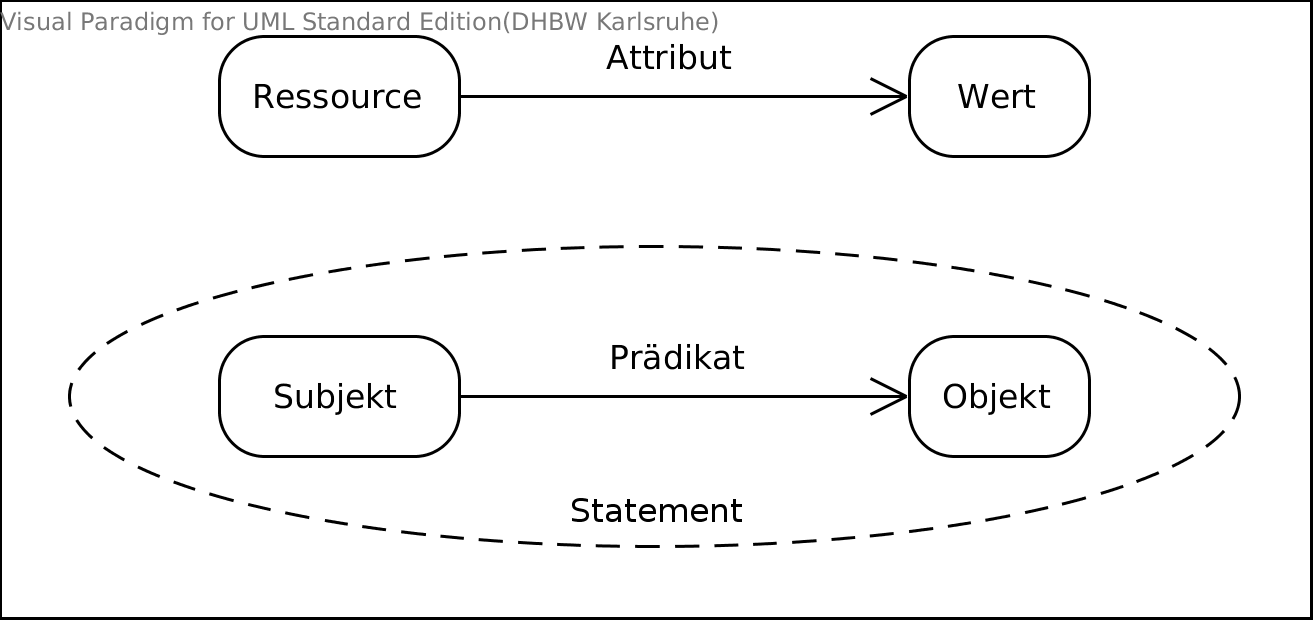
\includegraphics[width=8cm]{Bilder/RDF.png}
\caption{Struktur von \ac{RDF}}
\label{RDF Struktur}
\centering
\end{figure}

Mit Hilfe von \ac{RDF} kann also ausgesagt werden, dass eine Website "`www.beispiel.com"' ein Erstellungsdatum am 15.06.2015 hat.
Somit ergibt sich die Aufteilung:
\begin{itemize}
 \item Subjekt: www.beispiel.com
 \item Pr\"adikat: hat Erstellungsdatum
 \item Objekt: 15.06.2015
\end{itemize}

In XML w\"urde dieses Beispiel wie im Listing \ref{RDF in XML} aussehen.
\cite{Multimedia_retrieval}

\lstinputlisting[caption=RDF-Beispiel in XML, label=RDF in XML]{Code/RDF.xml}

\subsubsection{ANSI/NISO Z39.87-2006 (R2011)} \label{R2011}
Das ANSI/NISO Z39.87-2006 ist ein amerikanisches nationales Format, welches Bilddateien beschreibt. Es ist \"ahnlich aufgebaut wie \ac{Exif} und enth\"alt grundlegend die selben M\"oglichkeiten wie das im Abschnitt \ref{Exif} vorgestellte \ac{Exif}. \cite{NISO_Standard}

Da sich die Arbeit jedoch mit europ\"aischen Projekten und Organisationen besch\"aftigt, wird auf dieses Format hier nicht weiter eingegangen.
\section{Erstellung eines Datenkonzepts}
\subsection{Fachlich}
\subsection{Technisch}
\section{Technologievergleich}
\subsection{Alfresco}
\subsection{anderes ECM}
\subsection{anderes ECM}
\section{Implementierung}
\subsection{Schnittstelle}
\subsection{Backend}
\subsection{Frontend}


\newpage
\section{Abk�rzungsverzeichnis}
\begin{acronym}
%   \acro{SDK}{\emph{Software Development Kits}}
%   \acro{OHA}{\emph{Open Handset Alliance}}
%   \acro{IDE}{\emph{Integrierte Entwicklungsumgebung}}
%   \acro{ADT}{\emph{Android Development Tools}}
%   \acro{DVM}{\emph{Dalvik Virtual Machine}}
%   \acro{FME}{\emph{Funkmeldeempf\"anger}}
%   \acro{JIT}{\emph{Just in Time}}
%   \acro{ART}{\emph{Android Runtime}}
%   \acro{AOT}{\emph{Ahead-of-Time-Decodierung}}
%   \acro{API}{\emph{Application Programming Interface}}
  \acro{ECM}{\emph{Enterprise Content Management}}
  \acro{DMS}{\emph{Dokumentenmanagementsystem}}
  \acro{PoC}{\emph{Proof of Concept}}
  \acro{LUBW}{\emph{Landesanstalt f\"ur Umwelt, Messungen und Naturschutz Baden-W\"urttemberg}}
  \acro{GAA}{\emph{Gewerbeaufsicht Baden-W\"urttemberg}}
  \acro{REST}{\emph{Representational State Transfer}}
  \acro{FADO}{\emph{Fachdokumente Online}}
  \acro{DRS}{\emph{Document Retrieval System}}
  \acro{INSPIRE}{\emph{Infrastructure for Spatial Information in the European Community}}
  \acro{API}{\emph{Application Programming Interface}}
  \acro{EU}{\emph{Europ\"aische Union}}
  \acro{}{\emph{}}
%  \acro{KIT}{\emph{Karlsruher Instituts f�r Technologie}}
%  \acro{GDS}{\emph{Generic Data Services}}
% %  \acro{LSDF}{\emph{Large Scale Data Facility}}
%  \acro{OPM}{\emph{Objektorientierten Programmiermodell}}
%  \acro{SMD}{\emph{Strukturelle Metadaten}}
%  \acro{JSON}{\emph{JavaScript Object Notation}}
% %  \acro{HALO}{\emph{High Altitude and Long Range Research Aircraft}}
%  \acro{IAI}{\emph{Institut f�r Angewandte Informatik}}
%  \acro{JAXB}{\emph{Java Architecture for XML Binding}}
%  \acro{UDDE}{\emph{User Data Description Editor}}
%  \acro{AMD}{\emph{Anwendermetadaten}}
%  \acro{CG}{\emph{Class Generator}}
%  \acro{IG}{\emph{Interface Generator}}
\end{acronym}
\newpage
\section{Anhang} \label{Anhang}
\subsection{Metadaten der LUBW Fachsysteme} \label{Metadaten der LUBW Fachsysteme}
In den folgenden Abschnitten sind die Metadaten und Relationen der Untersuchten Dokumente in \ac{FADO} abgebildet.
\subsubsection{Metadaten des Fachsystems FADO / Urteile}
\begin{table}[ht]
\begin{center}
\begin{tabular}{|l|l|}
\hline
\textbf{Metadaten:} & \textbf{Werte:} \\ \hline
Fachsystem & Vorgabe \\ \hline
ID & Generiert \\ \hline
Titel & Freitext \\ \hline
Tenor & Freitext \\ \hline
Kommentar & Freitext \\ \hline
Orientierungssatz & Freitext \\ \hline
Norm & Freitext \\ \hline
Leitsatz & Freitext \\ \hline
Gericht & Freitext \\ \hline
Entscheidungsform & Freitext \\ \hline
Entscheidungsdatum & Datum \\ \hline
Aktenzeichen & Freitext \\ \hline
Vorgericht & Freitext \\ \hline
Nachgericht & Freitext \\ \hline
Sachverhalt & Freitext \\ \hline
Gr�nde & Freitext \\ \hline
Unsichtbar & Bool \\ \hline
ausblenden & Bool \\ \hline
\end{tabular}
\label{Metadaten der Urteile in FADO}
\caption{Metadaten der Urteile in FADO}
\end{center}
\end{table}

\begin{table}[ht]
\begin{center}
\begin{tabular}{|l|l|}
\hline
\textbf{Relationen:} & \textbf{Werte:} \\ \hline
Thema & Vorgabe \\ \hline
geh�rt zu Fachobjekt & Vorgabe \\ \hline
hat Schlagwort & Vorgabe \\ \hline
ist vom Typ & Vorgabe \\ \hline
enthalten in Fachsystem & Vorgabe \\ \hline
wird referenziert von & Vorgabe \\ \hline
\end{tabular}
\label{Relationen der Urteile in FADO}
\caption{Relationen der Urteile in FADO}
\end{center}
\end{table}

\newpage
\subsubsection{Metadaten des Fachsystems FADO / Forschungsvorhaben}

\begin{table}[!ht]
\begin{center}
\begin{tabular}{|l|l|}
\hline
\textbf{Metadaten:} & \textbf{Werte:} \\ \hline
Fachsystem & Vorgabe \\ \hline
ID & Generiert \\ \hline
Title & Freitext \\ \hline
Kurzbeschreibung & Freitext \\ \hline
Kommentar & Freitext \\ \hline
F�rderbereich & Freitext \\ \hline
Beginn & Datum \\ \hline
Ende & Datum \\ \hline
Projektnummer & Freitext \\ \hline
F�rderkennzeichen & Freitext \\ \hline
Unsichtbar & Bool \\ \hline
ausblenden & Bool \\ \hline
\end{tabular}
\label{Metadaten der Forschungsvorhaben in FADO}
\caption{Metadaten der Forschungsvorhaben in FADO}
\end{center}
\end{table}

\begin{table}[!ht]
\begin{center}
\begin{tabular}{|l|l|}
\hline
\textbf{Relationen:} & \textbf{Werte:} \\ \hline
Thema & Vorgabe \\ \hline
geh�rt zu Fachobjekt & Vorgabe \\ \hline
hat Abschlussbericht & Vorgabe \\ \hline
hat Forschungsberichtsblatt & Vorgabe \\ \hline
hat Projektskizze & Vorgabe \\ \hline
hat Schlagwort & Vorgabe \\ \hline
hat Zwischenbericht & Vorgabe \\ \hline
wird geleitet von & Vorgabe \\ \hline
wird referenziert von & Vorgabe \\ \hline
\end{tabular}
\label{Relationen der Forschungsvorhaben in FADO}
\caption{Relationen der Forschungsvorhaben in FADO}
\end{center}
\end{table}

\newpage
\subsubsection{Metadaten des Fachsystems FADO / Berichte}

\begin{table}[!ht]
\begin{center}
\begin{tabular}{|l|l|}
\hline
\textbf{Metadaten:} & \textbf{Werte:} \\ \hline
Fachsystem & Vorgabe \\ \hline
ID & Generiert \\ \hline
Titel & Freitext \\ \hline
Kurzbeschreibung & Freitext \\ \hline
Kommentar & Freitext \\ \hline
Kurztitel & Freitext \\ \hline
Untertitel & Freitext \\ \hline
Fachthema & Freitext \\ \hline
Herausgeber & Freitext \\ \hline
Redaktion & Freitext \\ \hline
Version & Freitext \\ \hline
Stand & Datum \\ \hline
Seitenzahl & Freitext \\ \hline
Seite (von-bis) & Freitext \\ \hline
Reihe & Freitext \\ \hline
Bandnummer & Freitext \\ \hline
ISSN & Freitext \\ \hline
ISBN & Freitext \\ \hline
Preis & Freitext \\ \hline
Medium & Freitext \\ \hline
Shoprelevant & Bool \\ \hline
Shoplink & URL \\ \hline
HTML-Datei & Data \\ \hline
PDF-Datei & Data \\ \hline
Weitere Datei & Data \\ \hline
Format dieser Datei & Freitext \\ \hline
Unsichtbar & Bool \\ \hline
ausblenden & Bool \\ \hline
\end{tabular}
\label{Metadaten der Berichte in FADO}
\caption{Metadaten der Berichte in FADO}
\end{center}
\end{table}

\begin{table}[!ht]
\begin{center}
\begin{tabular}{|l|l|}
\hline
\textbf{Relationen:} & \textbf{Werte:} \\ \hline
betrift Thema & Vorgabe \\ \hline
geh�rt zu Fachobjekt & Vorgabe \\ \hline
hat Autor & Vorgabe \\ \hline
hat Schlagwort & Vorgabe \\ \hline
ist vom Typ & Vorgabe \\ \hline
enthalten in Fachsystem & Vorgabe \\ \hline
ist Abschlussbericht von & Vorgabe \\ \hline
ist Forschungsberichtsblatt von & Vorgabe \\ \hline
ist Projektskizze von & Vorgabe \\ \hline
ist Zwischenbericht von & Vorgabe \\ \hline
wird referenziert von & Vorgabe \\ \hline
\end{tabular}
\label{Relationen der Berichte in FADO}
\caption{Relationen der Berichte in FADO}
\end{center}
\end{table}

\newpage
\subsubsection{Metadaten des DRS}

\begin{table}[htbp]
\begin{center}
\begin{tabular}{|l|l|}
\hline
\textbf{Metadaten:} & \textbf{Werte:} \\ \hline
G�ltigkeit & Vorgabe \\ \hline
Titel & Freitext \\ \hline
Aktenzeichen & Freitext \\ \hline
Kurz-Titel & Vorgabe \\ \hline
Dokumentart & Vorgabe \\ \hline
Herausgeber & Vorgabe \\ \hline
Erscheinungsort & Vorgabe \\ \hline
Handbuch & Vorgabe \\ \hline
Kapitel & Vorgabe \\ \hline
Fundstelle & Vorgabe \\ \hline
Fassung & Vorgabe \\ \hline
�nderung & Vorgabe \\ \hline
Gr��e & Zahl \\ \hline
Formate & Vorgabe \\ \hline
\end{tabular}
\label{Metadaten des DRS}
\caption{Metadaten des DRS}
\end{center}
\end{table}

Zu beachten ist hier, dass die Metadaten-Tags Fassung und \"Anderung zusammengesetzte Daten enthalten, wie es in der Abbildung \ref{Suchmaske DRS} zu sehen ist.

\newpage
\subsubsection{Metadaten des Bildarchivs}

\begin{table}[htbp]
\begin{center}
\begin{tabular}{|l|l|}
\hline
\textbf{Metadaten:} & \textbf{Werte:} \\ \hline
Objektart & Freitext \\ \hline
Objektname & Freitext \\ \hline
ID & Generiert \\ \hline
URL & URL \\ \hline
Dateityp & Vorgabe \\ \hline
Name & Freitext \\ \hline
Kurzname & Freitext \\ \hline
Erstellt am & Datum \\ \hline
Autor & Freitext \\ \hline
Besitzer & Besitzer \\ \hline
Bemerkung & Freitext \\ \hline
\end{tabular}
\label{Metadaten des Bildarchivs}
\caption{Metadaten des}
\end{center}
\end{table}

\newpage
\subsection{Metadaten der ICT-ENSURE} \label{Metadaten der ICT-ENSURE}
In den folgenden Abschnitten sind die Metadaten der Dokumente der \ac{ICT-ENSURE} zu finden. Diese werden hier in UML-Form abgebildet, was auch dem eigentlichen Datenmodell hinter \ac{ICT-ENSURE} entspricht. \cite{ICT-ENSURE_Bericht}

\begin{figure}[!ht]
\centering
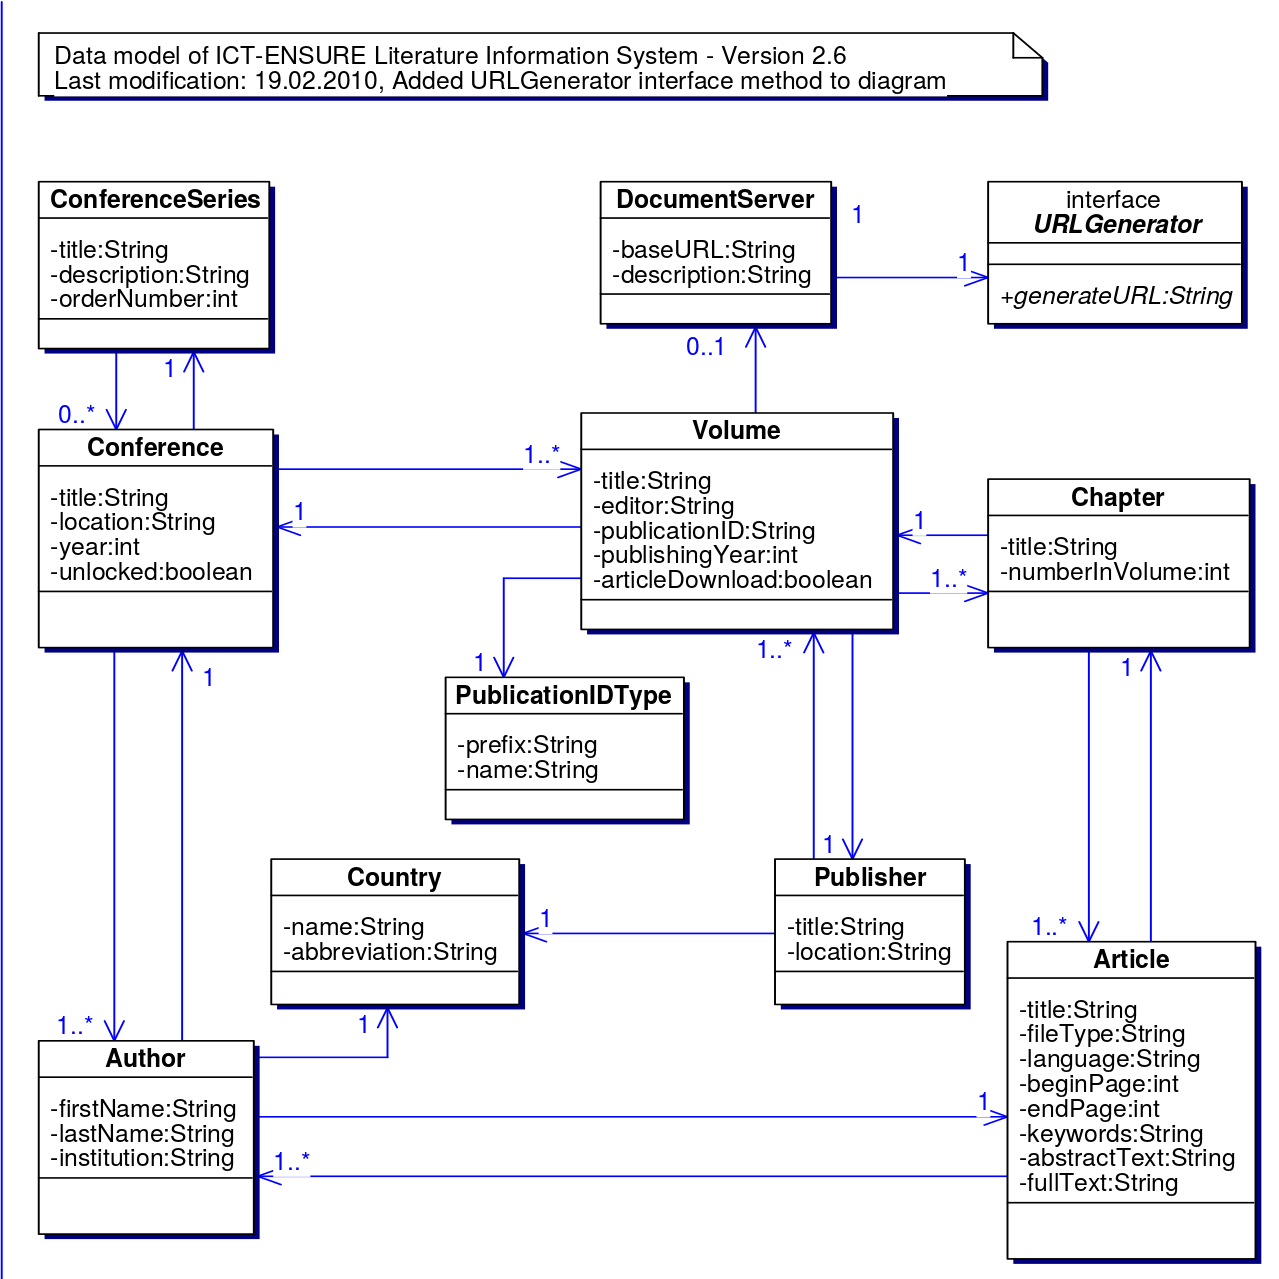
\includegraphics[width=15cm]{Bilder/Datenmodell_LitDB_V26_2010-03-11_Reduziert_fuer_Addendum.png}
\caption{Struktur von \ac{RDF}}
\label{RDF Struktur}
\centering
\end{figure}

% \subsubsection{Metadaten der Konferenzen}
% 
% \begin{table}[htbp]
% \begin{center}
% \begin{tabular}{|l|l|}
% \hline
% \textbf{Metadaten:} & \textbf{Werte:} \\ \hline
% Editor & Freitext (Mehrere Autoren) \\ \hline
% Publisher & Freitext (Bestehend aus Name und Ort) \\ \hline
% Year of Pblishing & Jahr \\ \hline
% ISBN & Freitext \\ \hline
% Conferenc & Freitext (Bestehend aus Titel, Ort, Jahr) \\ \hline
% \end{tabular}
% \label{Metadaten der Konferenzen von ICT-ENSURE}
% \caption{Metadaten der Konferenzen von ICT-ENSURE}
% \end{center}
% \end{table}
% 
% \subsubsection{Metadaten der Kapitel}
% 
% \begin{table}[htbp]
% \begin{center}
% \begin{tabular}{|l|l|}
% \hline
% \textbf{Metadaten:} & \textbf{Werte:} \\ \hline
% Editor & Freitext (Mehrere Autoren) \\ \hline
% Publisher & Freitext (Bestehend aus Name und Ort) \\ \hline
% Year of Pblishing & Jahr \\ \hline
% ISBN & Freitext \\ \hline
% Conferenc & Freitext (Bestehend aus Titel, Ort, Jahr) \\ \hline
% Editor & Freitext (Mehrere Autoren) \\ \hline
% \end{tabular}
% \label{Metadaten der Kapitel von ICT-ENSURE}
% \caption{Metadaten der Kapitel von ICT-ENSURE}
% \end{center}
% \end{table}
% 
% \subsubsection{Metadaten der Artikel}
% 
% \begin{table}[htbp]
% \begin{center}
% \begin{tabular}{|l|l|}
% \hline
% \textbf{Metadaten:} & \textbf{Werte:} \\ \hline
% Konferenz & Vorgabe \\ \hline
% Kapitel & Vorgabe \\ \hline
% Author & Freitext (ggf. Mehrere) \\ \hline
% Dateityp & Vorgabe \\ \hline
% Titel & Freitext \\ \hline
% Sprache & Freitext \\ \hline
% Beginn Seite & Zahl \\ \hline
% End Seite & Zahl \\ \hline
% Schl�sselw�rter & Freitext \\ \hline
% Abstract & Freitext \\ \hline
% Volltext & Freitext \\ \hline
% \end{tabular}
% \label{Metadaten der Vortr\"age von ICT-ENSURE}
% \caption{Metadaten der Vortr\"age von ICT-ENSURE}
% \end{center}
% \end{table}

\newpage
\listoffigures
\newpage
\listoftables
% Abk�rzungsverzeichnis
\newpage
\bibliographystyle{alpha}
% verzeichnis im DIN format
\bibliography{Quellen}
\end{document}
